\newpage
\section{2 семестр}
	\subsection*{1}
	Пусть есть окружности $S_1$ и $S_2$, угол между ними $\frac{2\pi}{3}$, найдите порядок композиции инверсий, то есть $\text{ord}(\text{inv}_{S_1} \circ \text{inv}_{S_2})$
	\begin{figure}[h]
		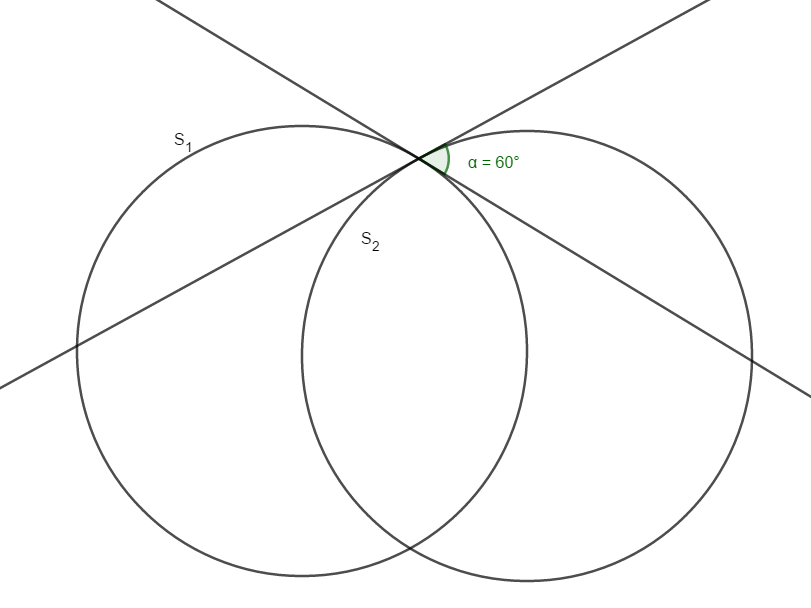
\includegraphics[width=0.5\linewidth]{pic3}
	\end{figure}
	
	\subsection*{2}
	Докажите, что инверсия -- элемент группы гомеоморфизмов $\mathbb{R}^2$, то есть $\text{inv} \in \text{Homeo}(\widehat{\mathbb{R}^2})$
	
	\subsection*{3}
	Даны две окружности $S_1$ и $S_2$\\
	Верно ли, что $\text{inv}_{S_{1}} \circ \text{inv}_{S_{2}} = \text{inv}_{S_{2}} \circ \text{inv}_{S_{1}}$
	\begin{figure}[h]
		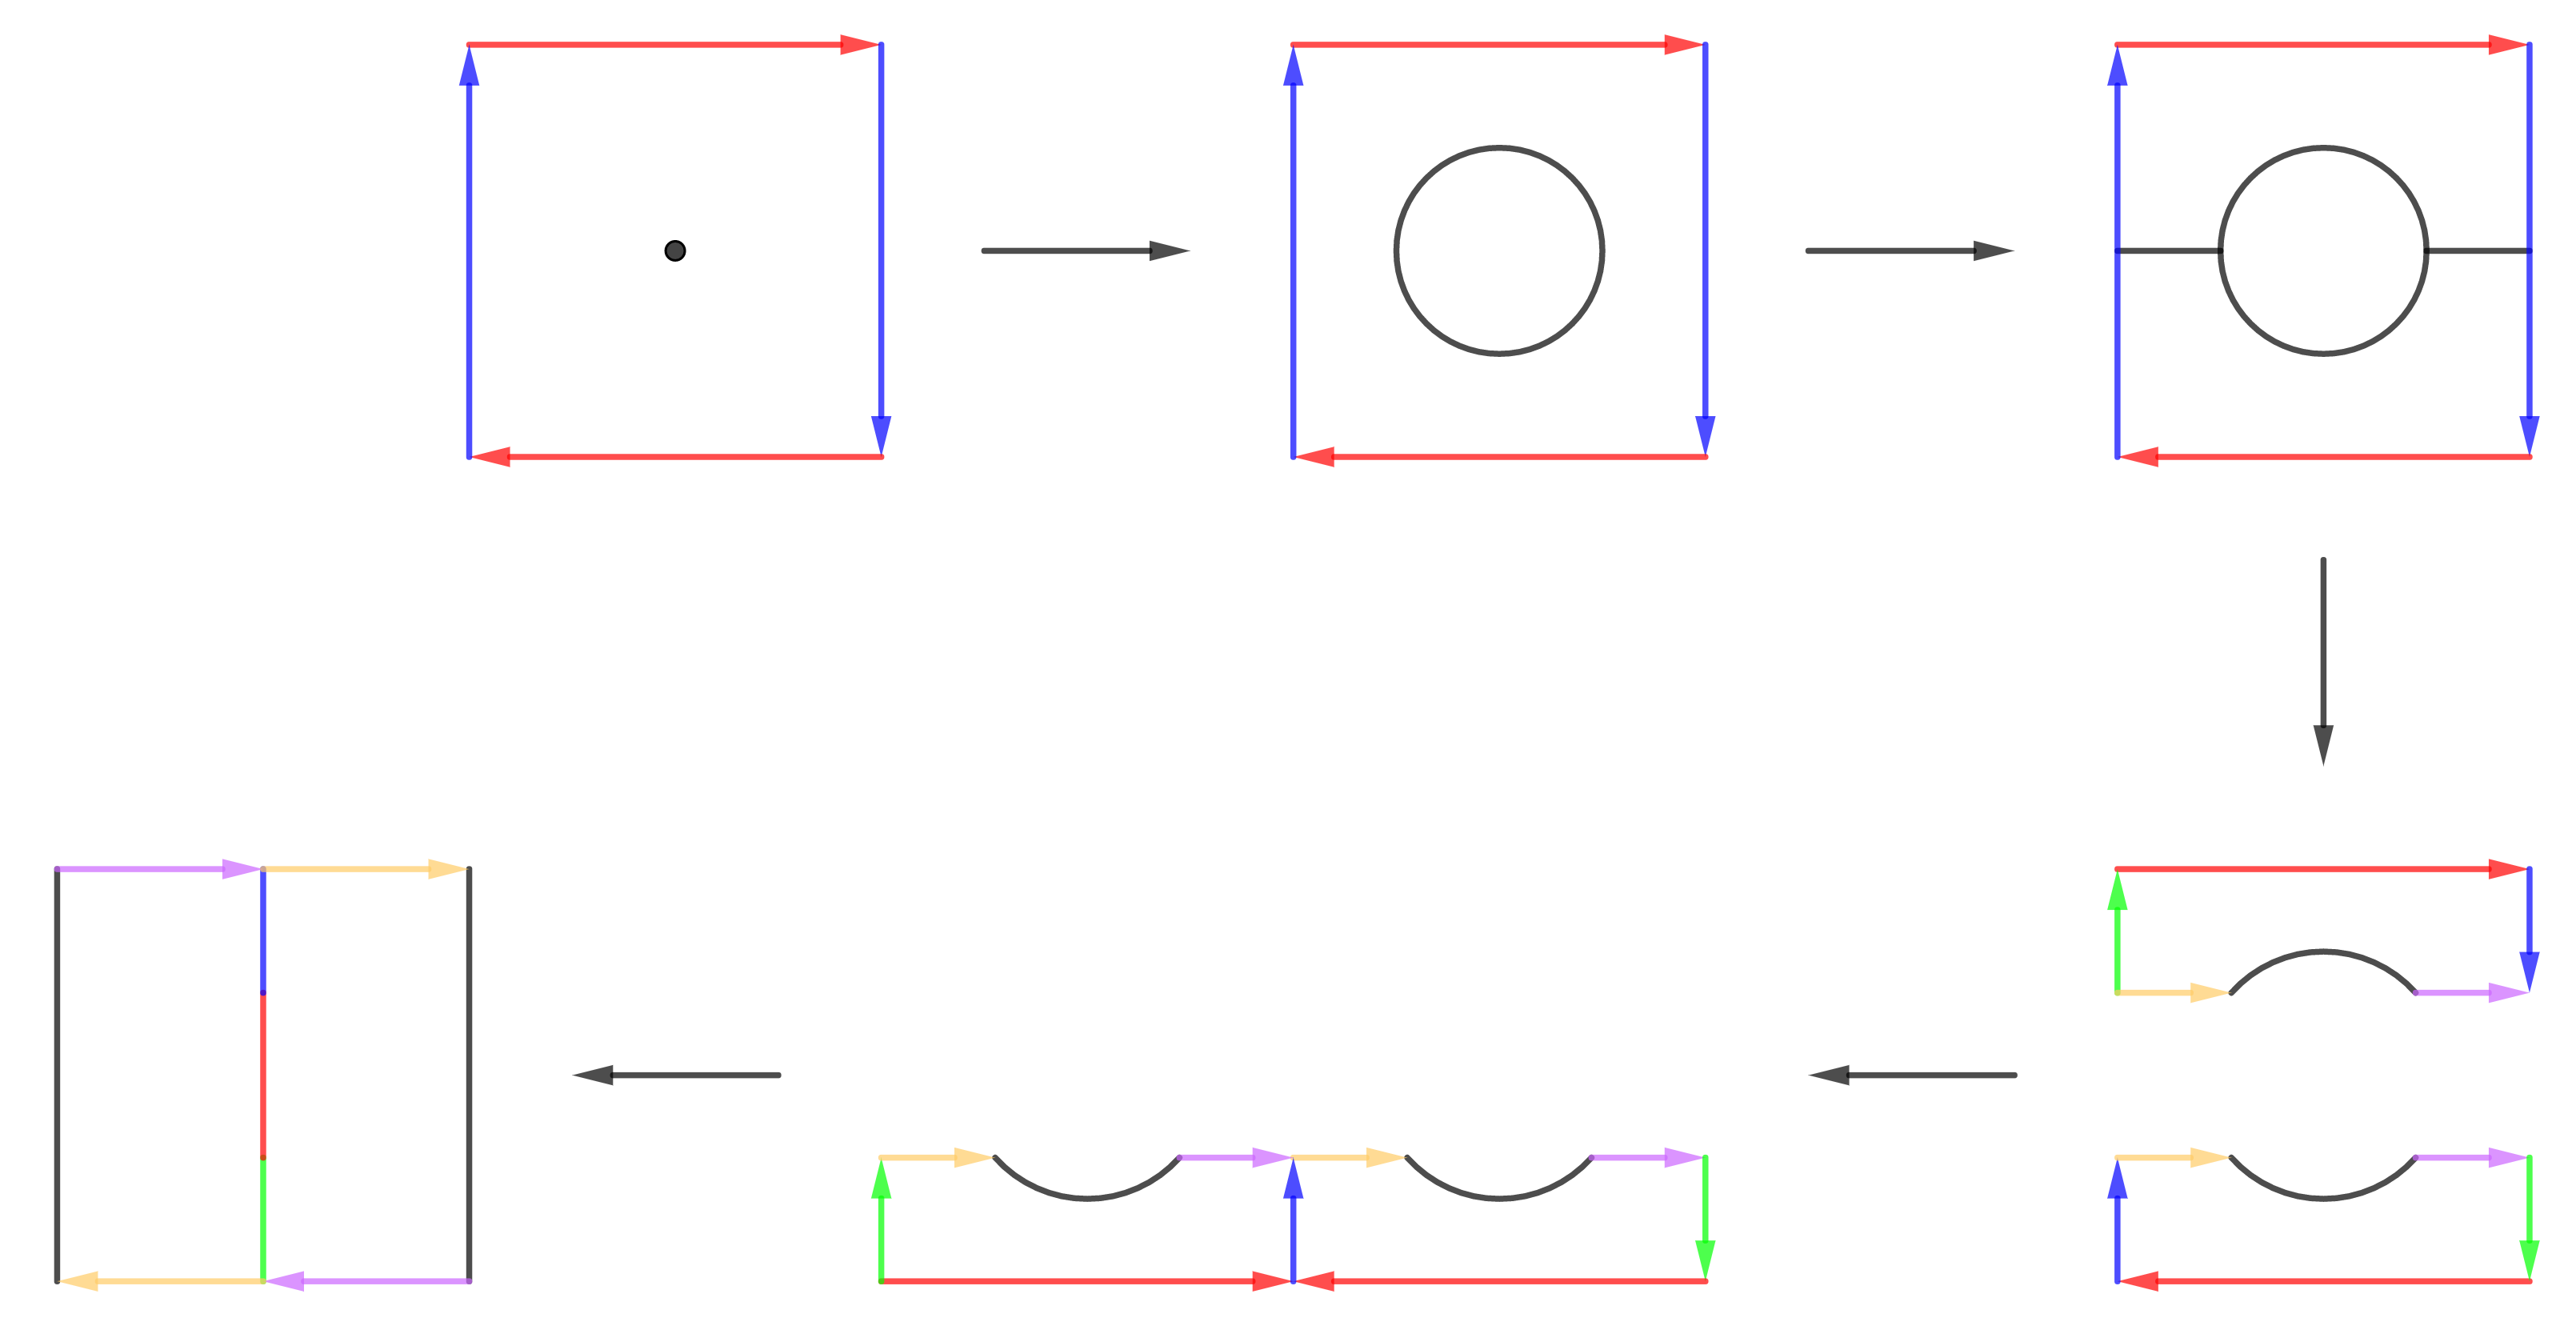
\includegraphics[width=0.5\linewidth]{pic4}
	\end{figure}
	
	\subsection*{4}
	Пусть на плоскости Лобачевского даны две различные точки $A$ и $B$, постройте преобразование, переводящее $A$ в $B$
	
	\subsection*{5}
	На плоскости Лобачевского найдите стабилизаторы точки $O$ в группе движений $G$, порожденной всеми инверсиями на этой плоскости $G = \langle \text{inv}_{l_{1}}, \text{inv}_{l_{2}},\: \ldots \rangle$
	
	\subsection*{6}
	Коэфициент искажения не может быть равен $0$, то есть:
	\begin{gather*}
		\text{Kg}(y) \ne 0\\
		\text{где}\quad \text{Kg}(y) = \lim\limits_{x \to y} \frac{|g(y) - g(x)|_{\text{e}}}{|y - x|_{\text{e}}}
	\end{gather*}
\newpage
	\subsection*{7}
	Как построить прямую перпендикулярную данным двум
	\begin{figure}[h]
		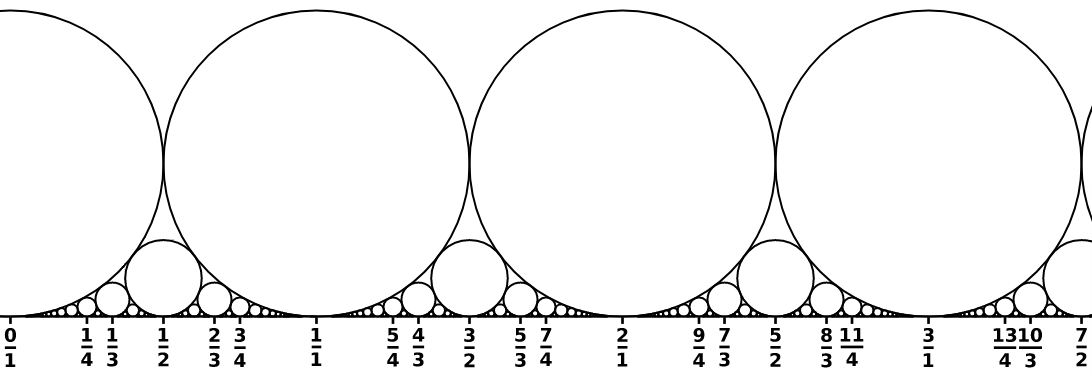
\includegraphics[width=0.35\linewidth]{pic5}
	\end{figure}
	
	\subsection*{8}
	Как построить перпендикуляр из точки на прямую
	\begin{figure}[h]
		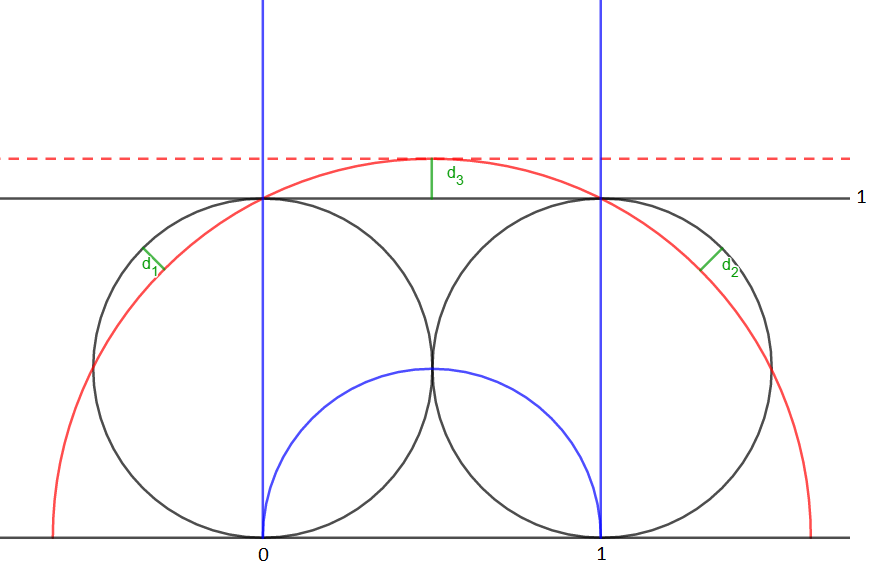
\includegraphics[width=0.35\linewidth]{pic6}
	\end{figure}

	\subsection*{9}
	Докажите, что минимальнй путь из точки A в точку B -- прямая
	\begin{figure}[h]
		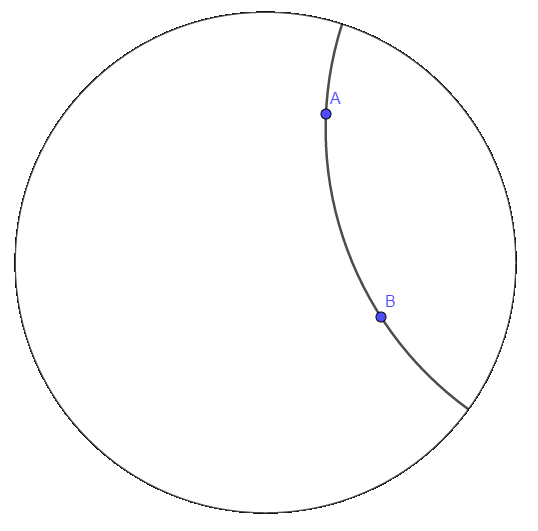
\includegraphics[width=0.35\linewidth]{pic7}
	\end{figure}
\newpage
	\subsection*{10}
	Докажите, что все существующие движения на $H^{2}$ разбиваются на 3 группы, и что дпугих движений нет.\\
	Движения:
	\begin{enumerate}
		\item[элиптические:] единственная неподвижная точка внутри, 0 на границе 
		\item[параболические:] единственная неподвижная точка на границе, 0 внутри
		\item[гиперболические:] 2 неподвижных точки на границе, 0 внутри
	\end{enumerate}
	\subsection*{11}
	Найдите длину окружности в гиперболической плоскости в зависимости от радиуса
	\begin{figure}[h]
		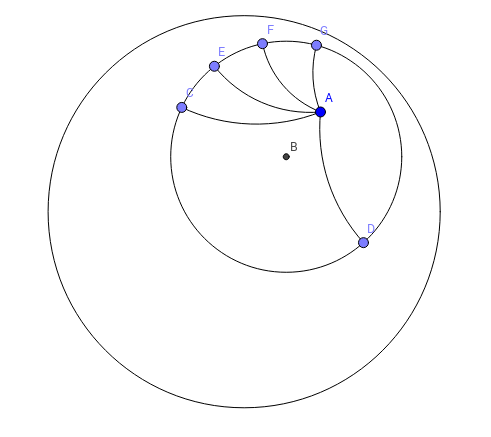
\includegraphics[width=0.35\linewidth]{pic8}
	\end{figure}
	\subsection*{12}
	Найдите площадь круга в гиперболической плоскости в зависимости от радиуса
	
	\subsection*{13}
	Докажите, что группа порождённая четным числом инверсий изоморфна $\text{PSL}(2,\mathbb{R})$
	
	\subsection*{14}
	Докажите, что с точностью до сопряженности все матрицы отличные от $E$ в $\text{SL}(2,\mathbb{R})$ делятся на три типа:
	\begin{enumerate}
		\item[(1)] $|\text{tr}(A)| > 2$, задающие гиперболическое преобразование
		\item[(2)] $|\text{tr}(A)| = 2$, задающие параболическое преобразование
		\item[(3)] $|\text{tr}(A)| < 2$, задающие элиптическое преобразование
	\end{enumerate}
	
	\subsection*{15}
	Найдите формулу выражающую расстояние от точки до прямой в $H^{2}$ и распишите все возможные её значения
	\begin{figure}[h]
		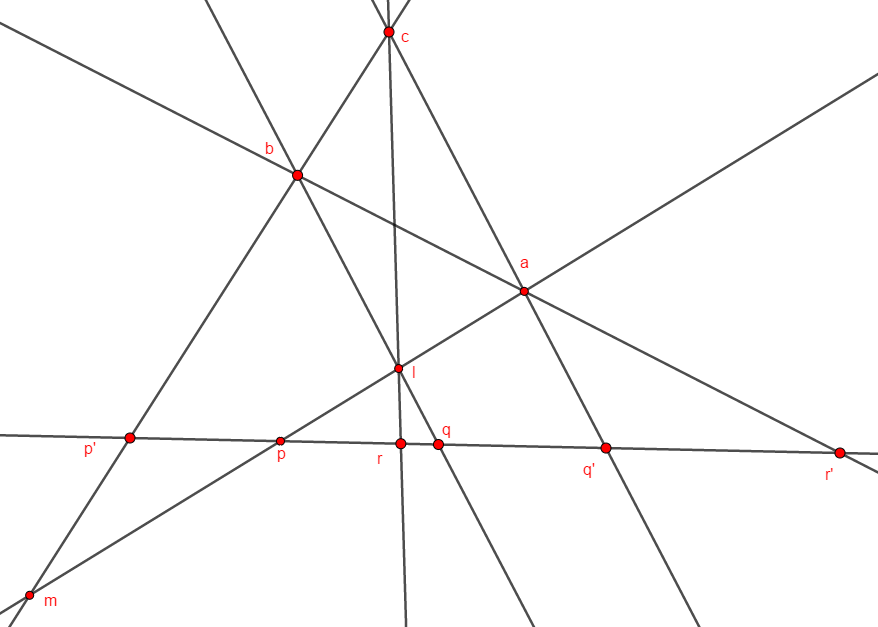
\includegraphics[width=0.35\linewidth]{pic9}
	\end{figure}
		
	\subsection*{16}
	Найдите формулу выражающую расстояние от точки до орицикла в $H^{2}$ и распишите все возможные её значения
		
	\subsection*{17}	
	Найдите формулу выражающую расстояние от орицикла до орицикла в $H^{2}$ и распишите все возможные её значения
	\begin{figure}[h]
		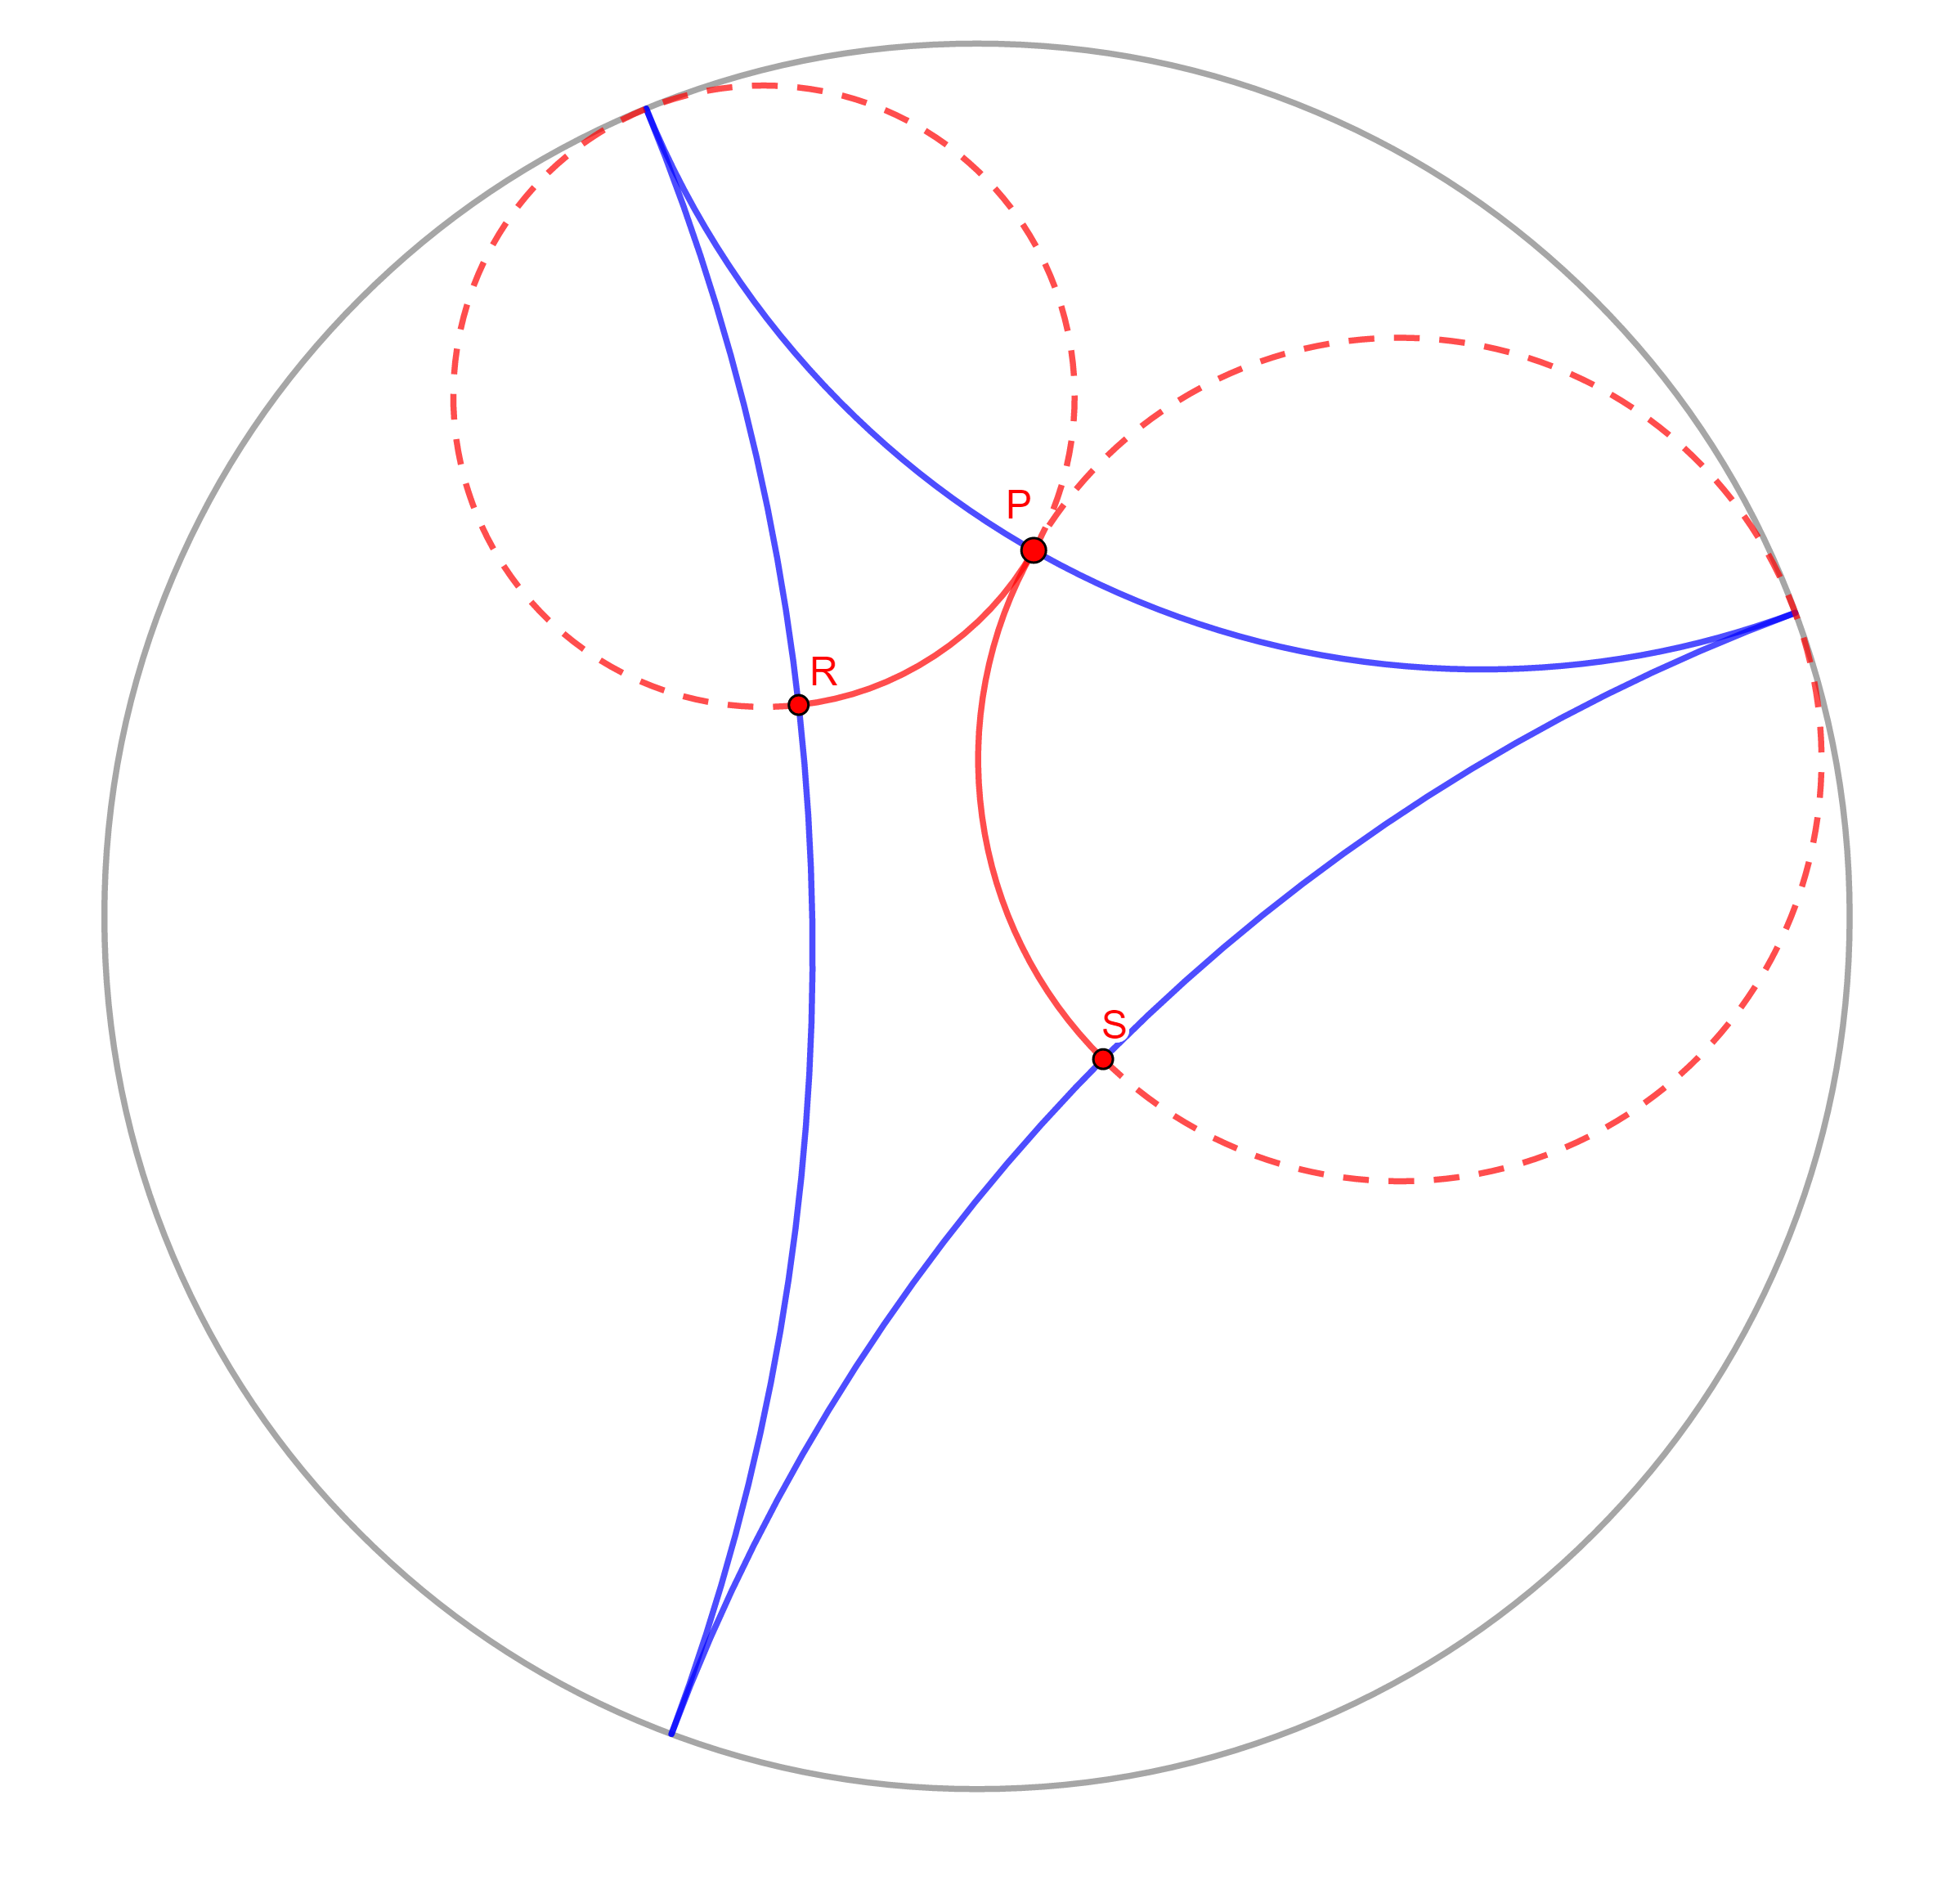
\includegraphics[width=0.4\linewidth]{pic11}
	\end{figure}